\section{Programmering av blokker}
\thispagestyle{fancy}

%Skriv OM:
%Programmering av IEC Blokker (MB,MA,SBE,SBV) 
%+ fb blokker (fbTimer, fbAnalougeAlarm, fbCAC)
%- Til appendiks, Heile kode for t.d. fbTimer, fbCAC osv

\subsection{Monitor Analogue}

\gls{MA} funksjonsblokka er brukt for skalering, visning, overvåking og alarmhandtering av analoge inngangsvariablar i ein prosess.
Funksjonsblokka inneheld supression og blokking funksjonalitet.

VI bruker \gls{MA} funksjonsblokka er brukt i programmet for å overvåke analoge trykknivågivarar samt å skalere og vise desse som ein fyllingsgrad i prosent.

\begin{figure}[htbp]
    \centering
    \begin{subfigure}[b]{0.45\textwidth}
        \centering
        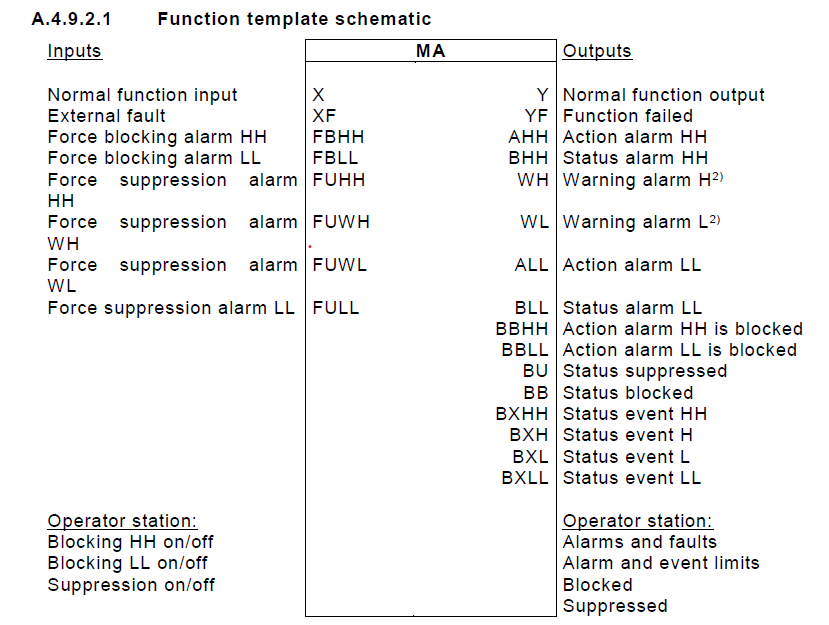
\includegraphics[width=1\textwidth]{Bilder/MABlokkIEC.png}
        \caption{IEC}\label{fig:Monitor Analogue blokk IEC}
    \end{subfigure}
    \hfill
    \begin{subfigure}[b]{0.45\textwidth}
        \centering
        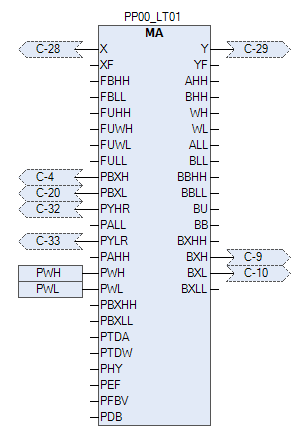
\includegraphics[width=0.7\textwidth]{Bilder/MABlokkIProgrammet.png}
        \caption{Bruk i programmet}\label{fig:Monitor Analogue blokk i programmet}
    \end{subfigure}
    \caption{Monitor Analogue}\label{fig:Monitor Analogue}
\end{figure}


% Skrive litt om blokka sin funksjonalitet
% Korleis me brukte blokkene i programmet.

\begin{figure}[htbp]
    \centering
    \begin{subfigure}[b]{0.45\textwidth}
        \centering
        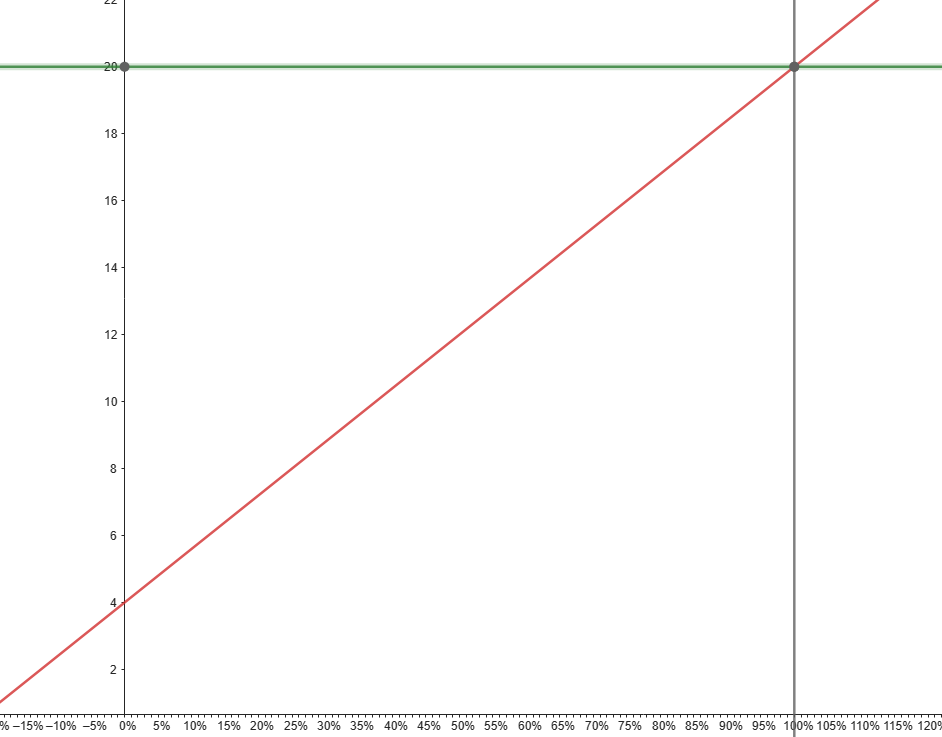
\includegraphics[width=1\textwidth]{Bilder/4_20mA_Scaling.png}
        \caption{Skalering av mA mot prosent}\label{fig:Skalering av mA mot prosent}
    \end{subfigure}
    \hfill
    \begin{subfigure}[b]{0.45\textwidth}
        \centering
        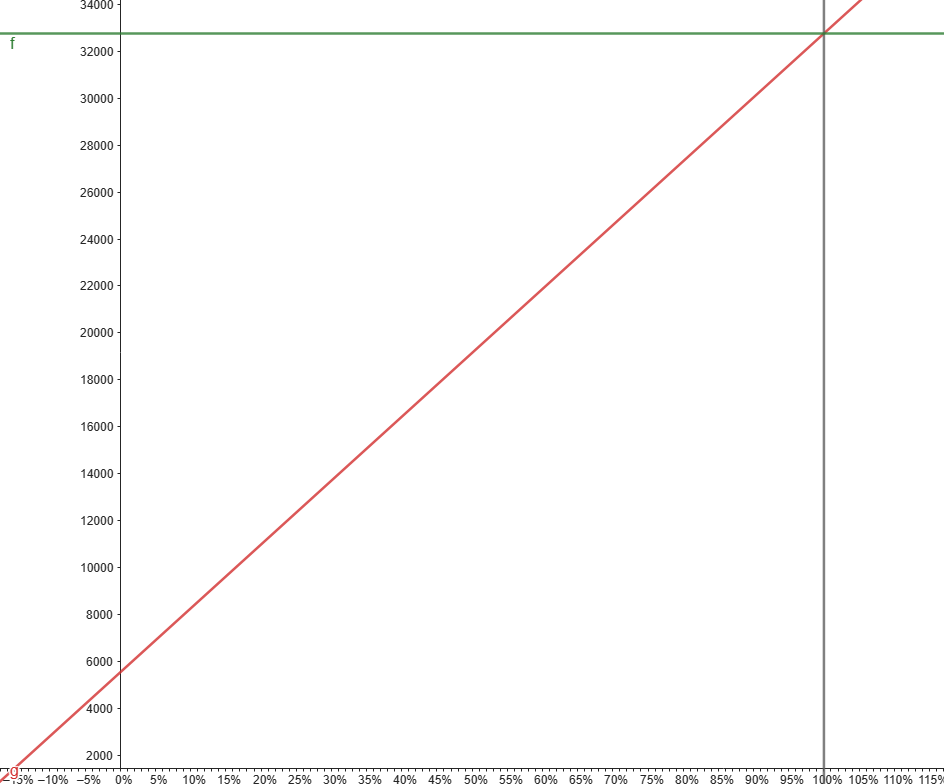
\includegraphics[width=0.95\textwidth]{Bilder/27327_prosent_Scaling.png}
        \caption{Skalering av prosent til verdi}\label{fig:Skalering av prosent til verdi}
    \end{subfigure}
    \caption{Dei forskjellige skaleringane av inngangssignal}\label{fig:Skalering av prosent til verdi}
\end{figure}